%----------------------------------------------------------------------------------------
%	Section: Minerva
%----------------------------------------------------------------------------------------
\section{Minerva}

\begin{figure}[h]
    	\centering
    		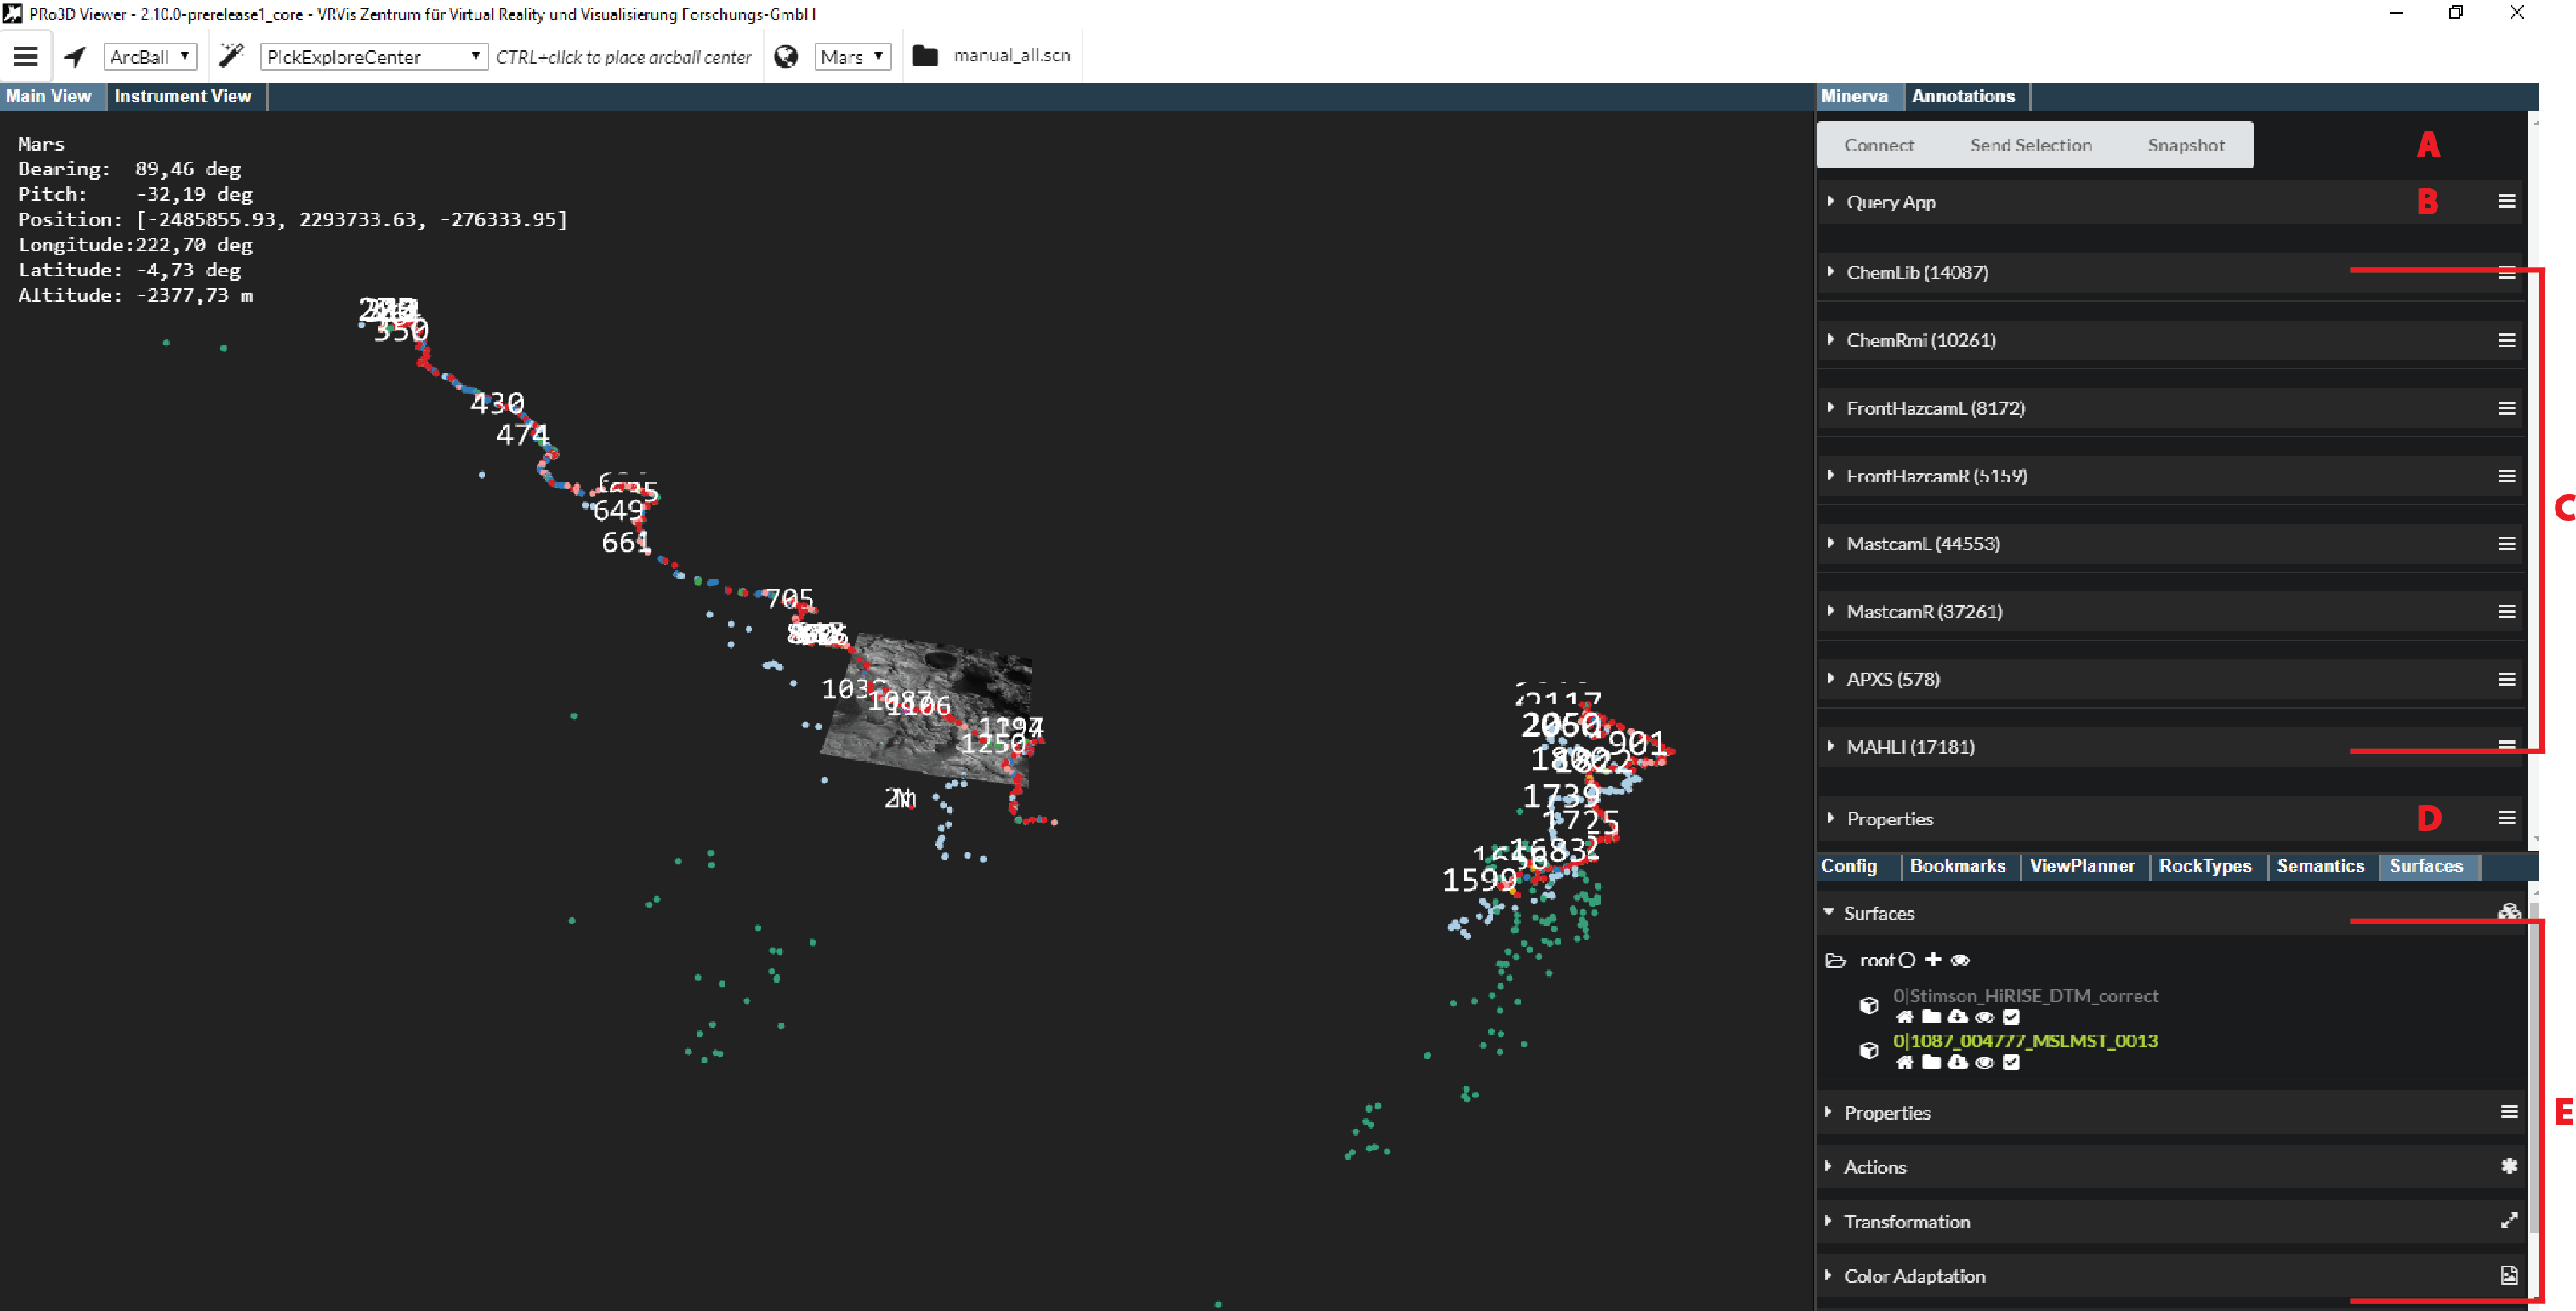
\includegraphics[width=1\textwidth]{pics/MinervaAI.png}
    	\caption[Start Minerva]{The Minerva Application. The Main View (left) shows the surface data with the products. There are different interaction possibilities for the products in the Minerva tab (right). A: Visplore communication, B: Query App to reduce the shown products by the mean of different criteria, C: Product listing, D: Properties of the last selected product, E: Surface tab.  }
    	\label{fig:StartMinerva}
   \end{figure}

%----------------------------------------------------------------------------------------
%	SubSection: Start Minerva
%----------------------------------------------------------------------------------------
\subsection{Start Minerva}
\label{sec:startMinerva}

Before you start the Minerva Application make sure that the \textbf{dump.csv} file is in the \textbf{\path{Release\netcoreapp2.0\MinervaData}} folder.
Then start the viewer by clicking the PRo3D.exe as described in Section~\ref{sec:startViewer}. The Minerva data from the dump.csv file is loaded and the products are listed in the ``Minerva'' tab as shown in Figure~\ref{fig:StartMinerva} C.  Load the surface data as described in Section~\ref{sec:addSurface}.
How to explore and adjust the surfaces is described in Section~\ref{sec:surfaces}.
You can save the scene as described in Section~\ref{sec:addSurface}.

%----------------------------------------------------------------------------------------
%	SubSection: Minerva Features
%----------------------------------------------------------------------------------------
\subsection{Minerva Features}
\label{sec:minervaFatures}

%----------------------------------------------------------------------------------------Visplore
\subsubsection{Visplore}

Visplore is a powerful visual analytics tool that allows the handling of huge and heterogeneous data and provides different perspectives onto the data that help finding causalities and allow an easy examination of the data's plausibility. 
For this project an interface was implemented that allows an interconnected workflow between PRo3D and Visplore.
To communicate with Visplore use the tree buttons shown in Figure~\ref{fig:StartMinerva} A:
\begin{itemize}
	\item \textbf{Connect:} Connect to Visplore.
	\item \textbf{Send Selection:} Send the selected products to Visplore.
	\item \textbf{Snapshot:} Send a snapshot of the MainView to the Visplore MapView.
\end{itemize}
For more information how to use Visplore for Minerva, please refer to the Visplore manual.

%----------------------------------------------------------------------------------------Query App
\subsubsection{QueryApp}
	
	\begin{figure}[h]
    	\centering
    		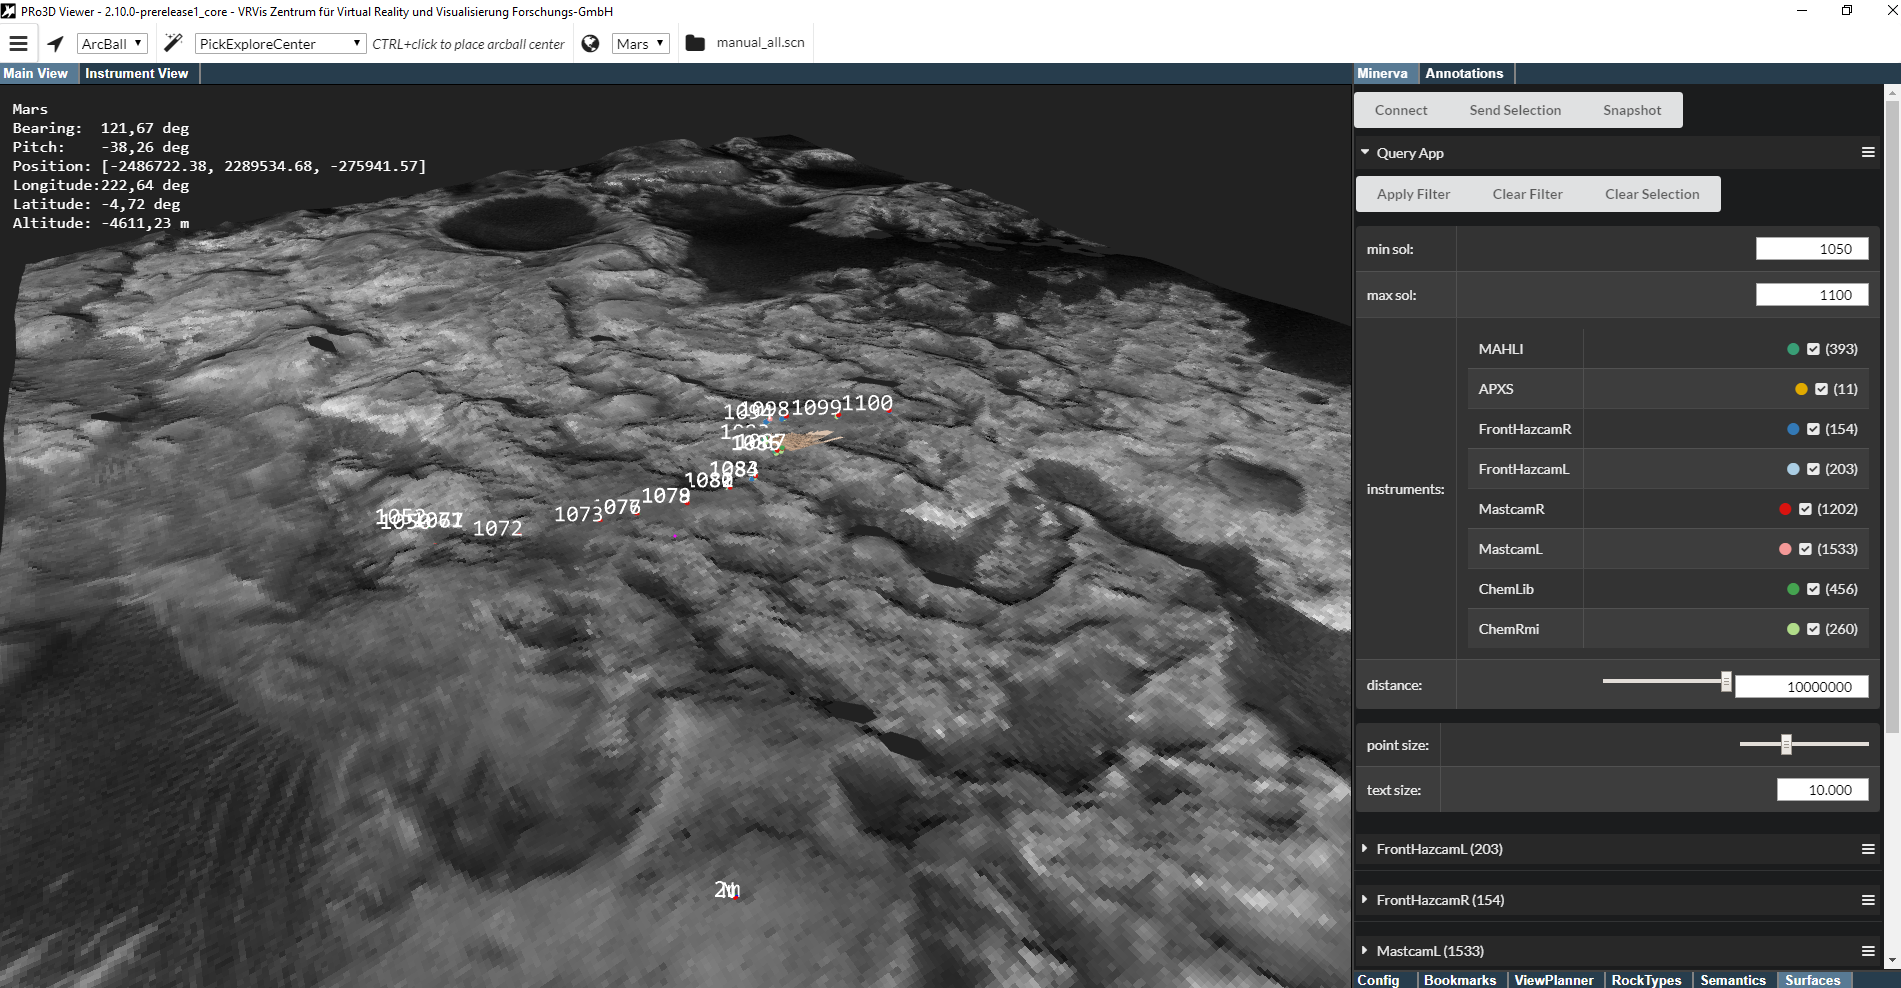
\includegraphics[width=1\textwidth]{pics/QueryApp.png}
    	\caption[Query App]{The Query App (right).}
    	\label{fig:QueryApp}
   \end{figure}

The Query App provides the possibility to cut down the number of shown products by the mean of different criteria. These criteria are:
\begin{itemize}
	\item \textbf{min- and max sol:} All products with sol numbers in the given range are shown.
	\item \textbf{instruments:} Only the products with checked instruments are shown.
	\item \textbf{distance:} The distance between the camera location and the shown products is less than the entered distance value.
\end{itemize}
You can use one ore more criteria and press the \textbf{``ApplyFilter''} button in top of the Query App menu. Now only the filtered products are shown. Change the queries and click ``ApplyFilter'' again to change the shown products. To get all products click the \textbf{``ClearFilter''} button. 
You can also change the \textbf{point size} of the rendered products in the Main View, and the \textbf{text size} of the shown sol numbers.

%----------------------------------------------------------------------------------------Product Listing
\subsubsection{Product Listing and Selection}
\label{sec:selection}

\begin{figure}[h]
				\centering
					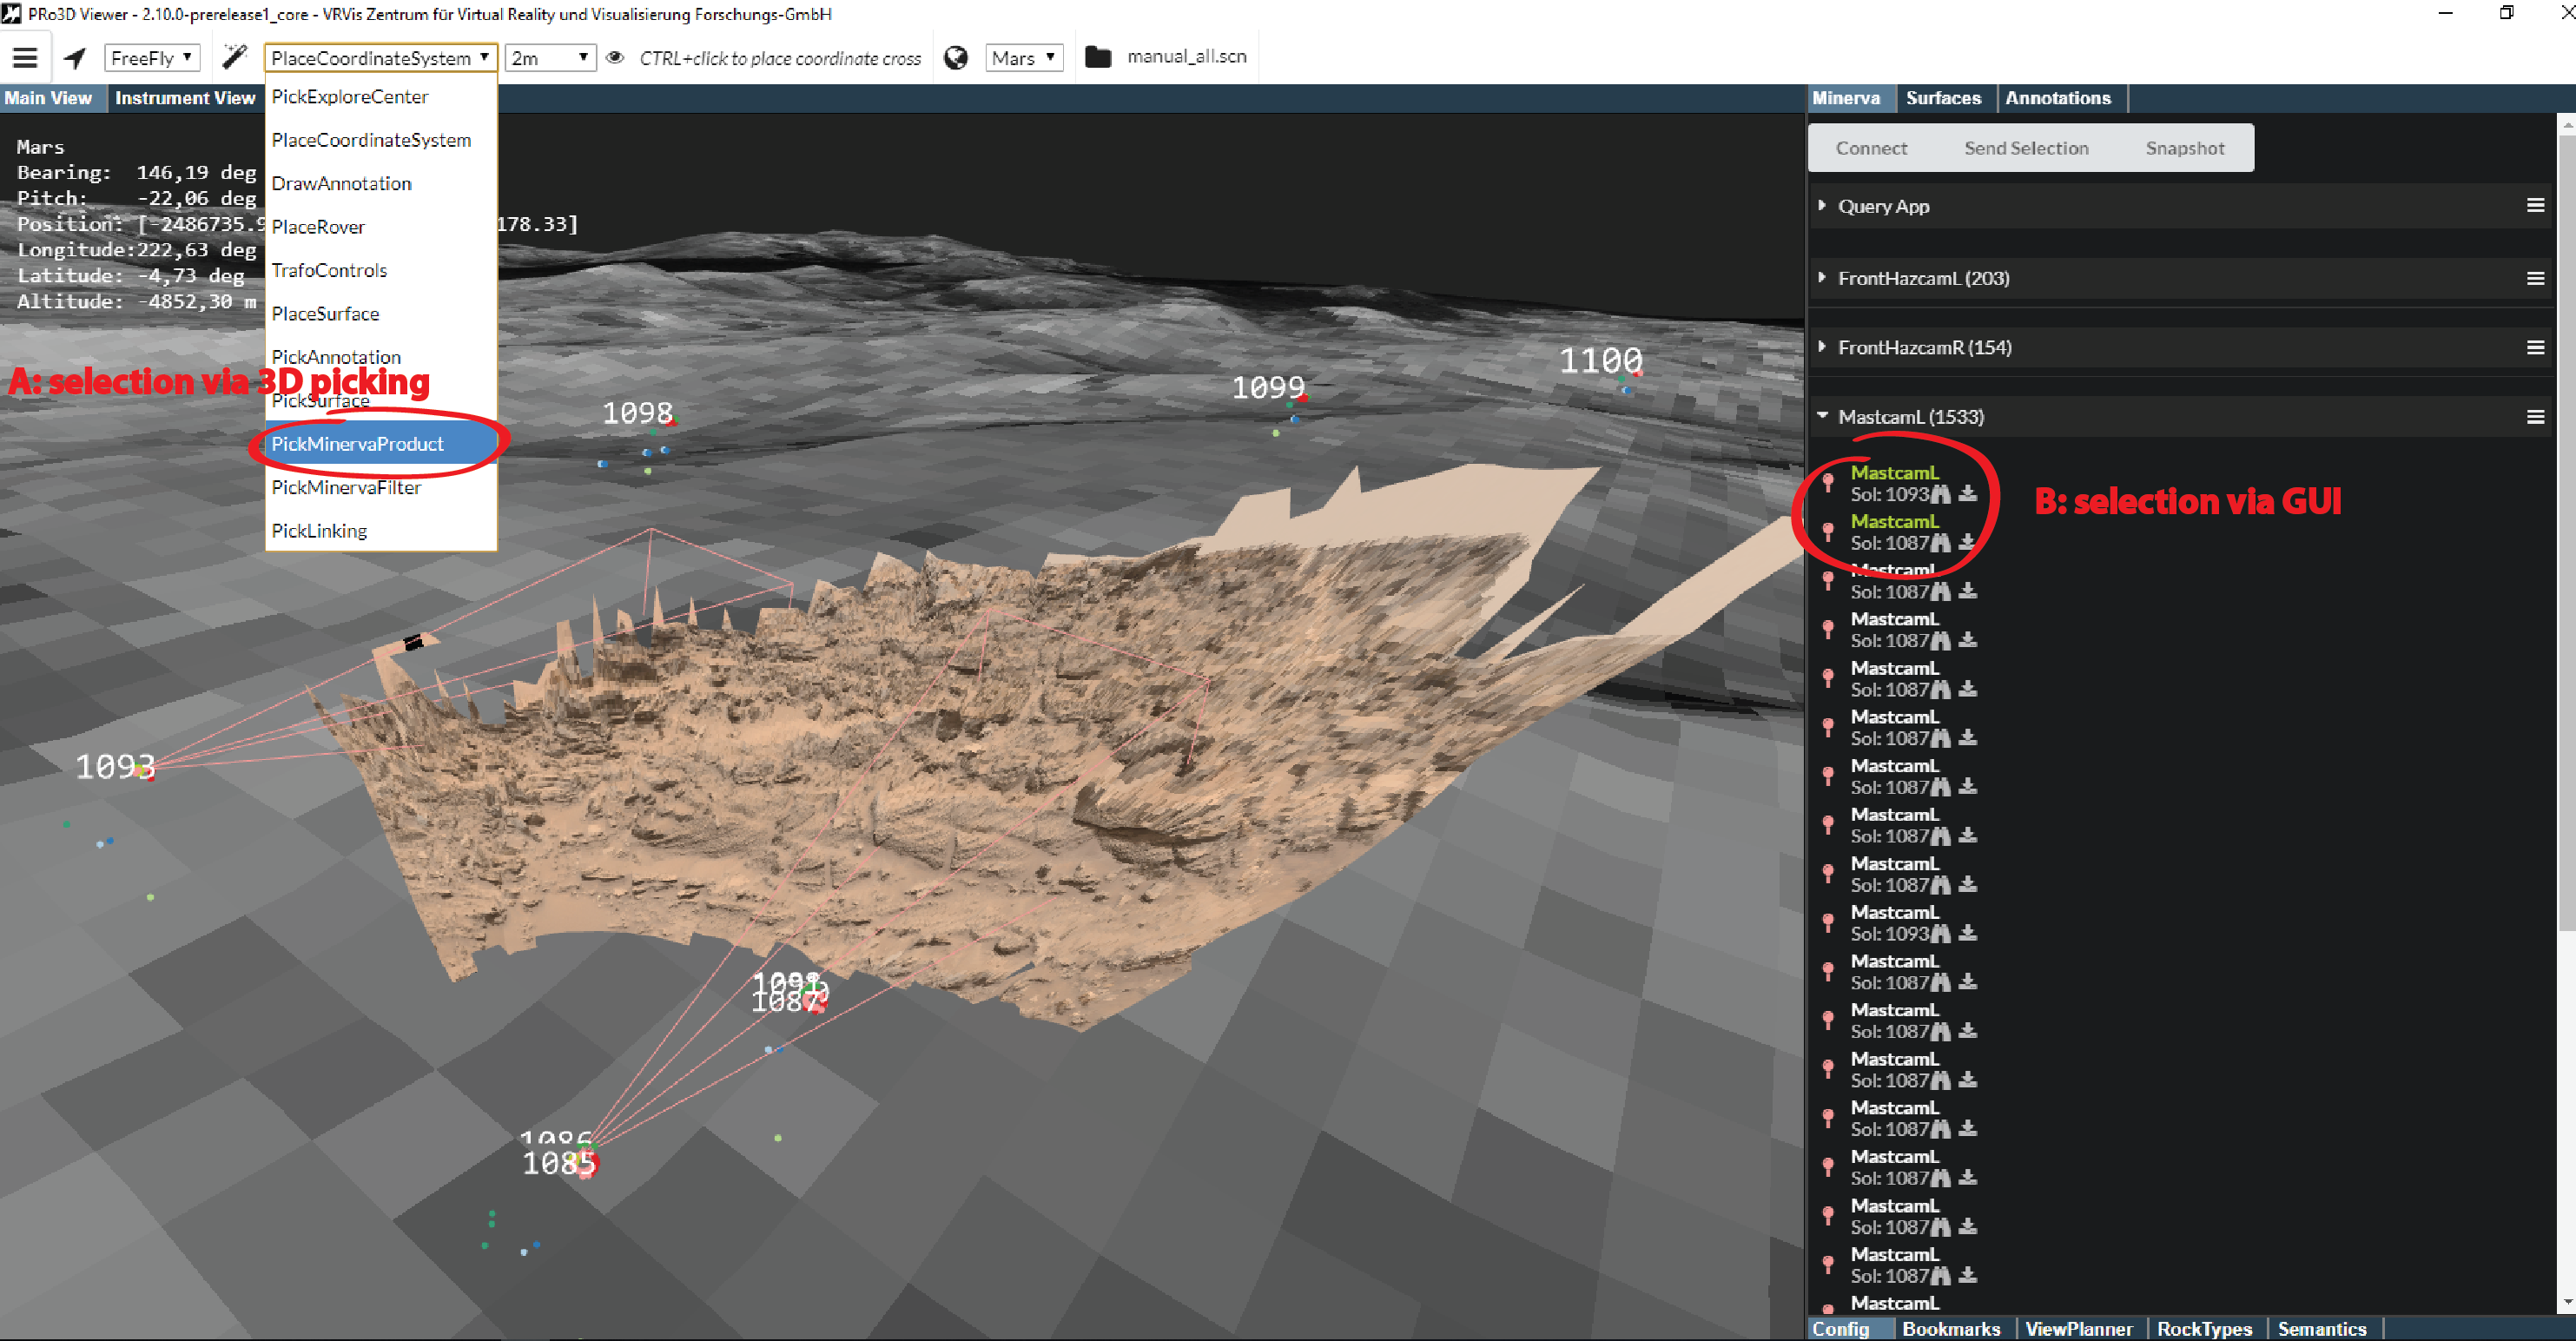
\includegraphics[width=1\textwidth]{pics/ListingAI.png}
				\caption[Product Listing]{The products are grouped by instruments. A product can either be selected in the listing (B) or in the Main View (A). }
				\label{fig:ProductListing}
		 \end{figure}
		
The products are grouped in the gui by their instruments (Figure~\ref{fig:StartMinerva} C) where the first 20 products for each instrument are listed.
You can select single products by clicking on the products's name, which turns its color to green. Or you can set ``PickMinervaProduct'' in the actions menu (Figure~\ref{fig:ProductListing}), press CTRL+LMB and pick the product in the main view. Then you can see the product's properties in the properties panel, described in the next Section~\ref{sec:productProps}. 

\begin{figure}[h]
				\centering
					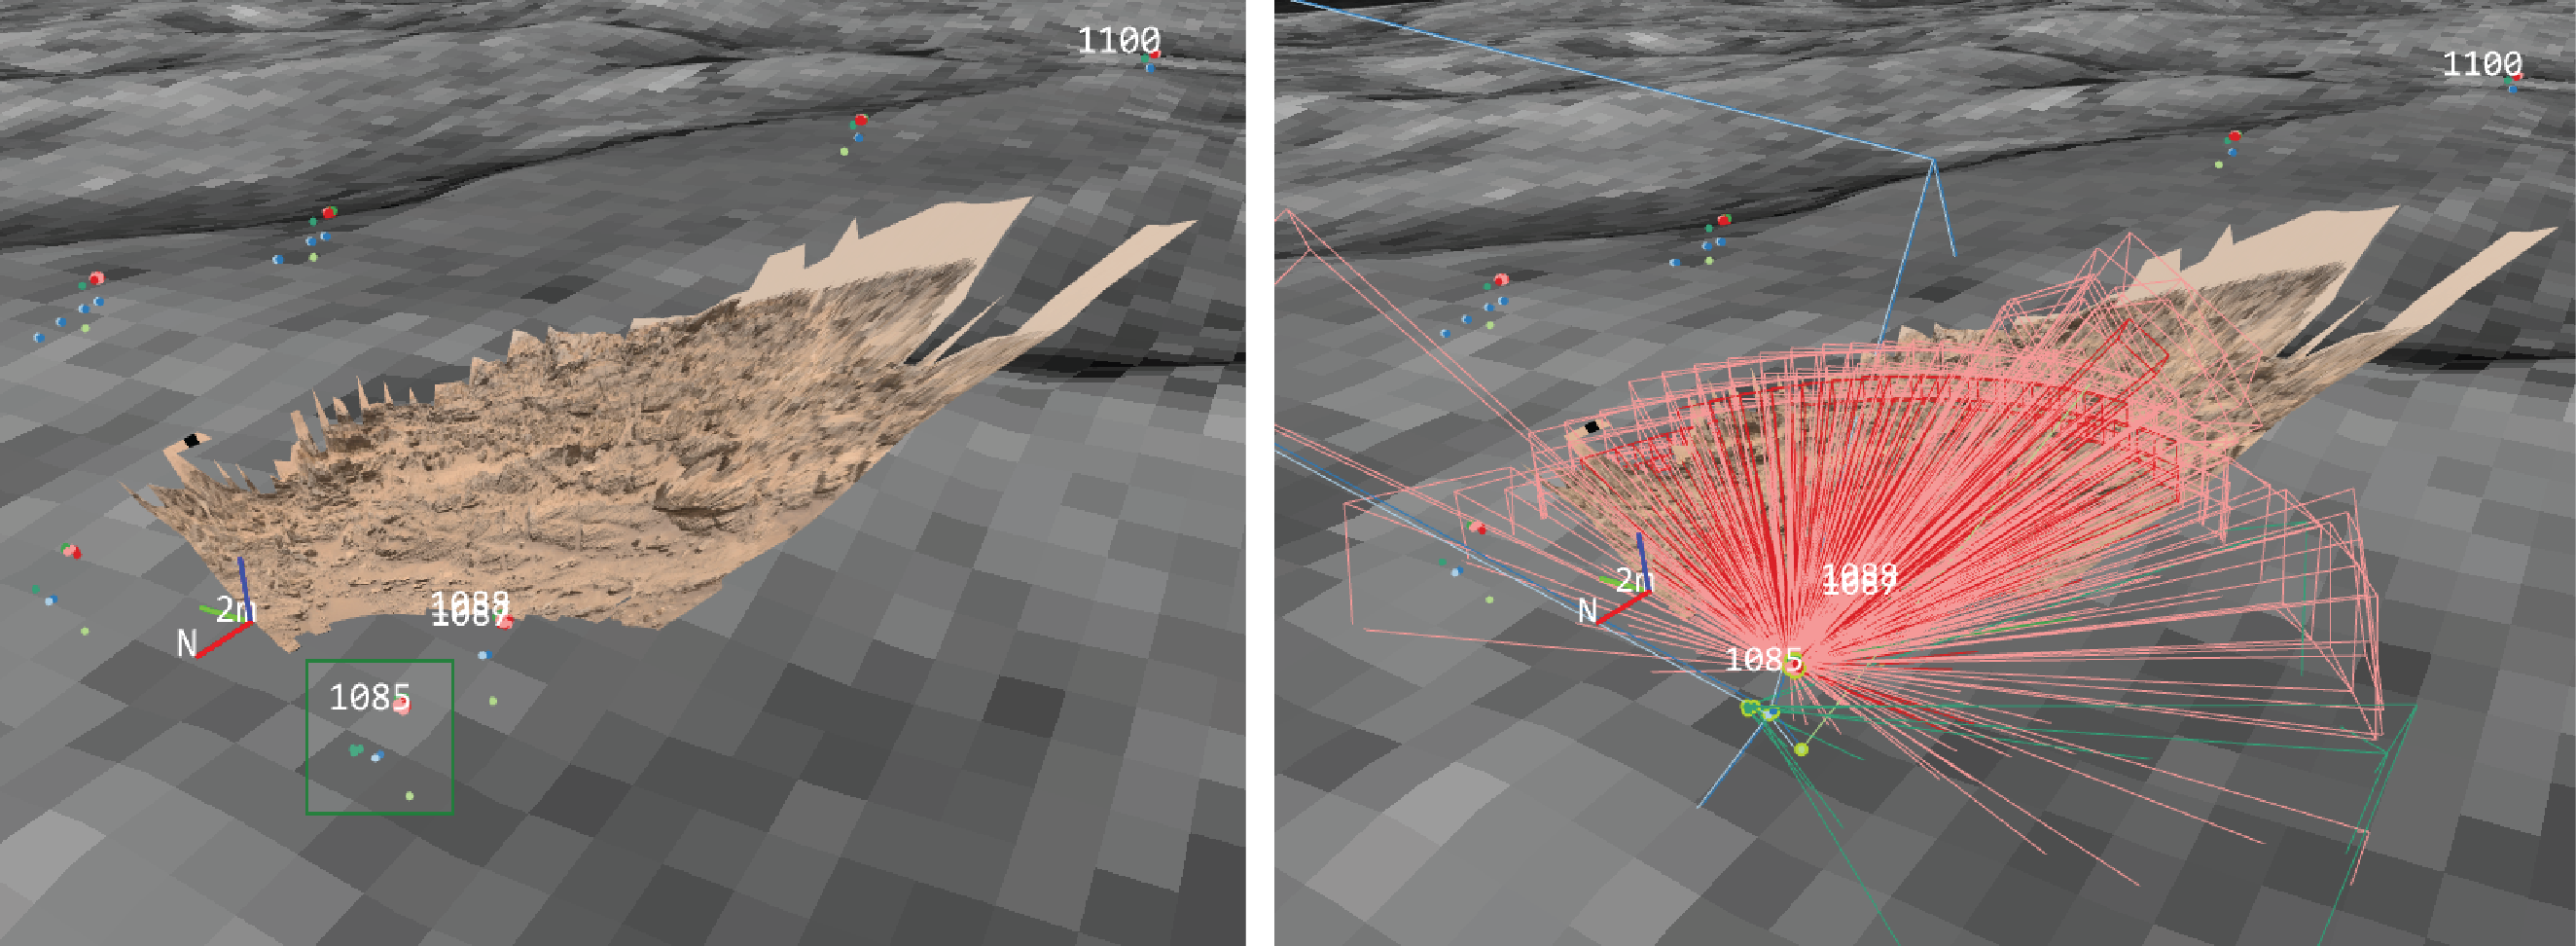
\includegraphics[width=1\textwidth]{pics/MultiSelAI.png}
				\caption[Multi Selection]{A rectangle is spanned over multiple products (left). All products selected by the rectangle (right).}
				\label{fig:MultiSel}
		 \end{figure}
		
It is also possible to select multiple products. Press SHIFT+LMB and drag a rectangle (Figure~\ref{fig:MultiSel} left). When you release the LMB, all products in this area are selected (Figure~\ref{fig:MultiSel} right). \\
Under the products's name is a little menu:
\begin{itemize}
  \item \textbf{The Sol Number}
	\item \textbf{FlyTo}: A click on the button triggers a FlyTo animation.
	\item \textbf{GetTif}: Downloads the product's tif image.
\end{itemize}

	
	
%----------------------------------------------------------------------------------------Product Properties
\subsubsection{Product Properties}
\label{sec:productProps}

\begin{figure}[h]
				\centering
					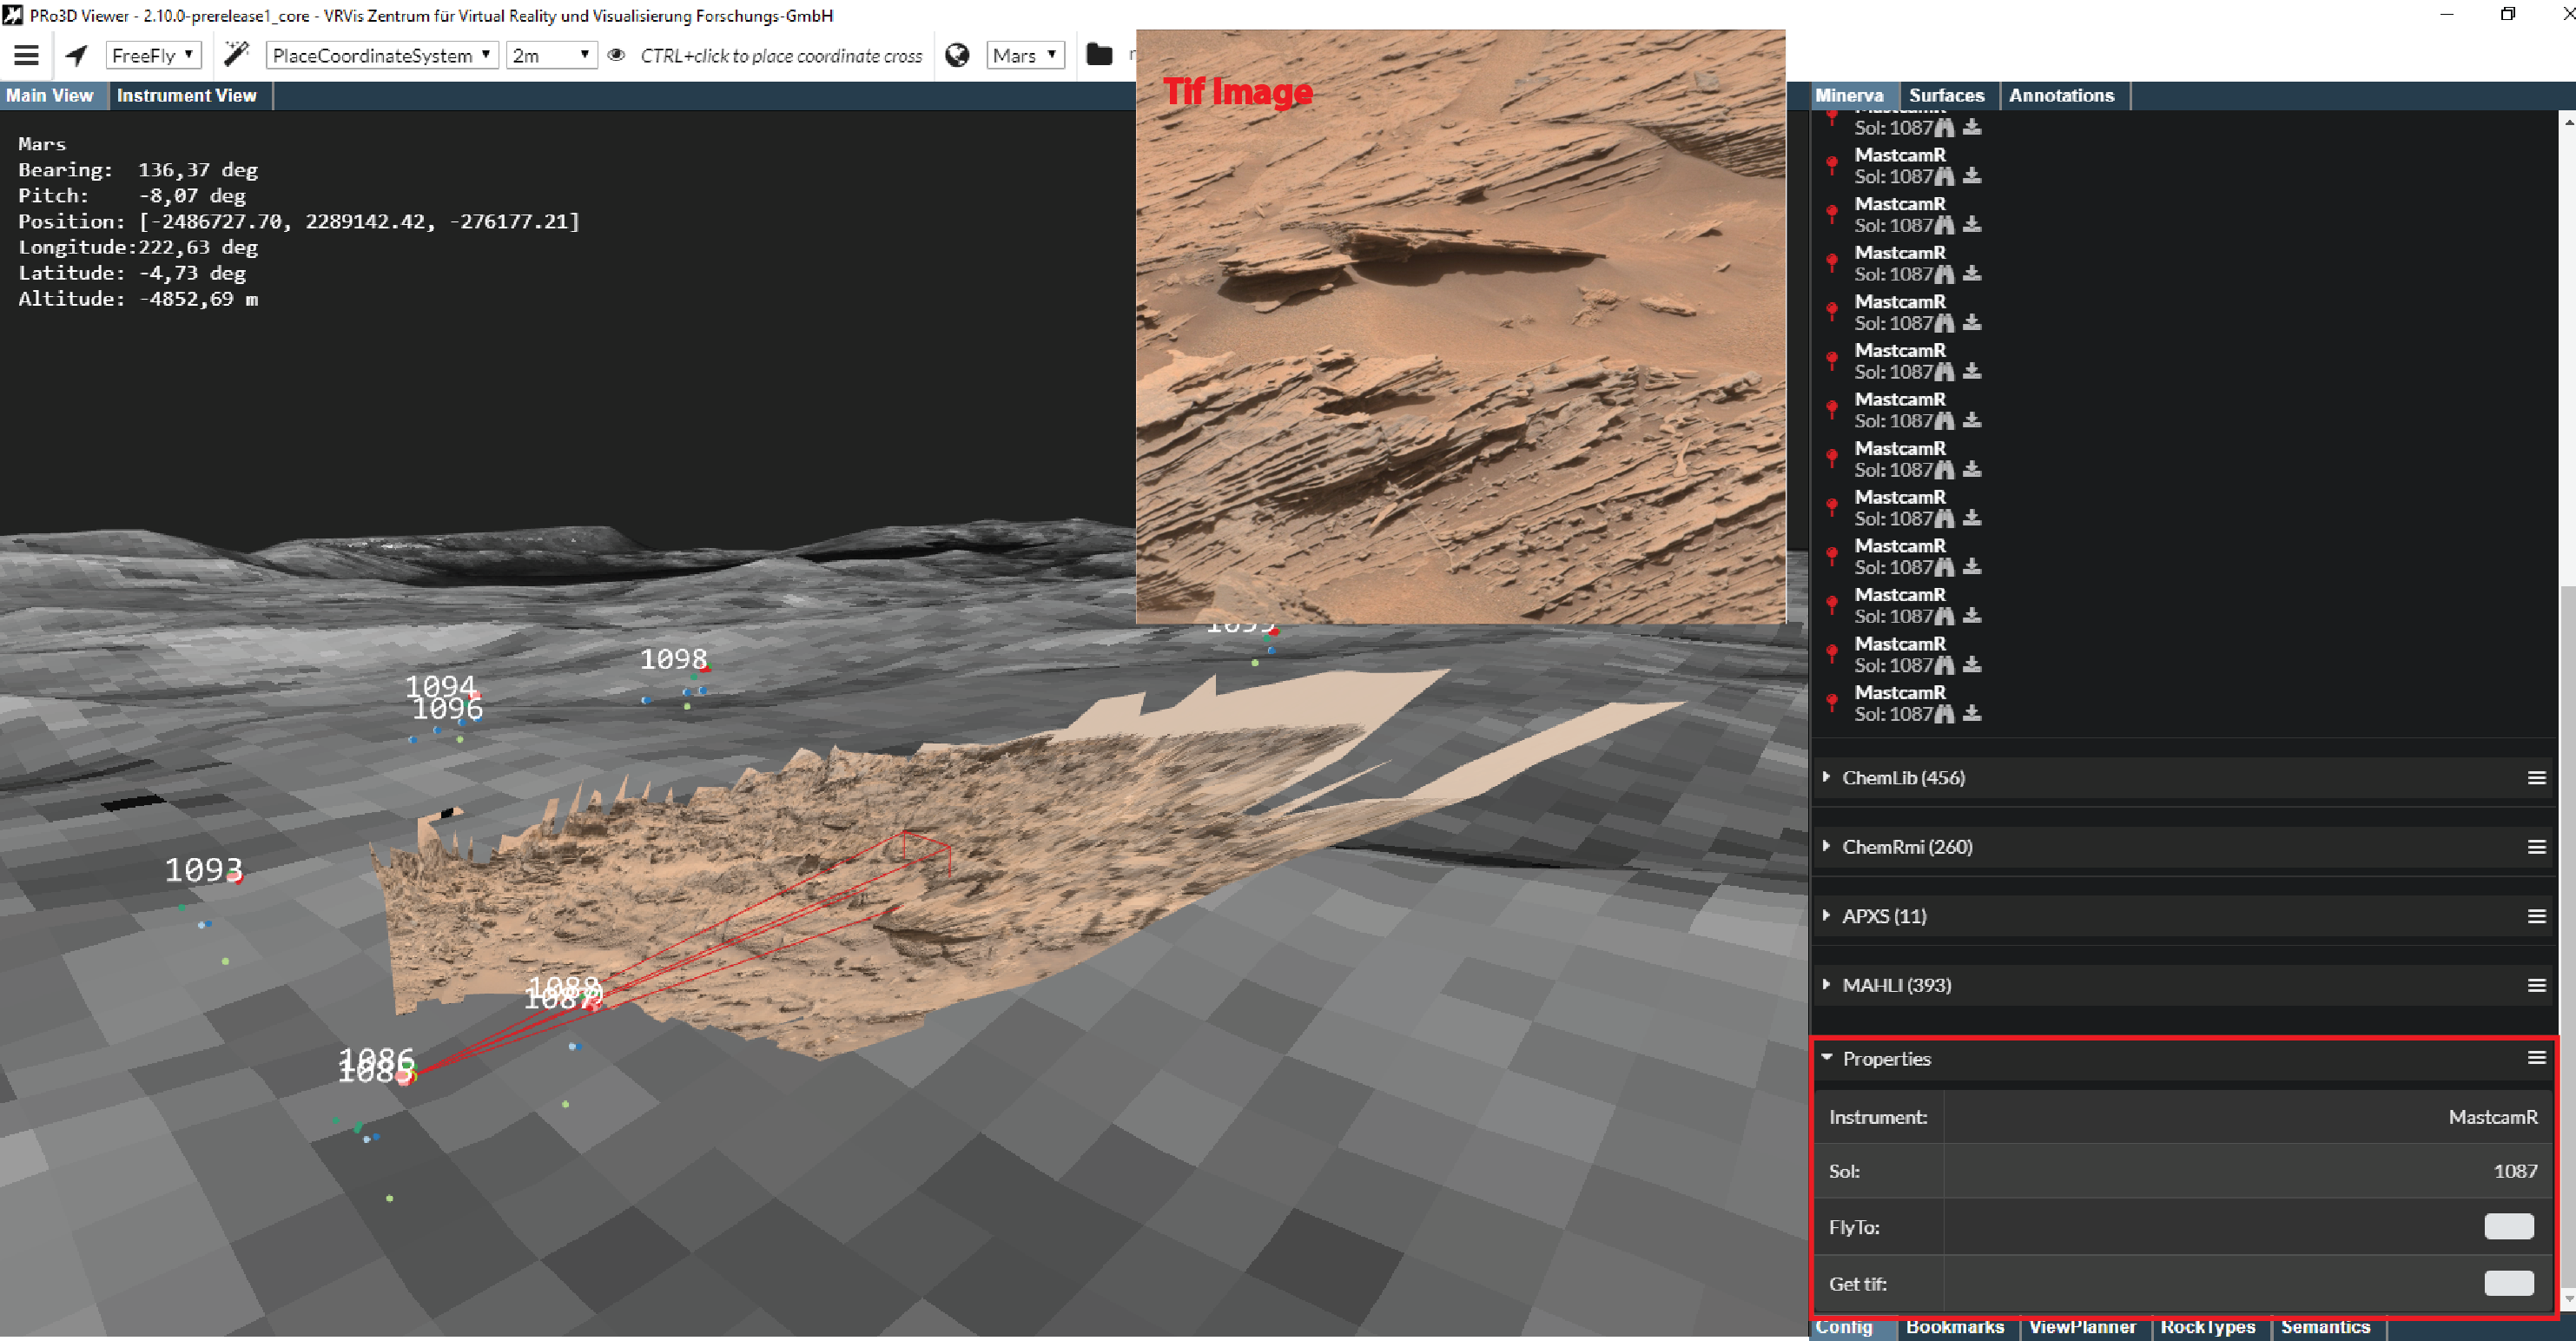
\includegraphics[width=1\textwidth]{pics/PropertiesAI.png}
				\caption[Product Properties]{The properties panel shows the sol number and provides interactions for the last selected product.}
				\label{fig:ProductProperties}
		 \end{figure}
		
The properties panel (Figure~\ref{fig:StartMinerva} D and Figure~\ref{fig:ProductProperties}) shows
\begin{itemize}
  \item \textbf{The Sol Number}
	\item \textbf{FlyTo}: A click on the button triggers a FlyTo animation.
	\item \textbf{GetTif}: Downloads the product's tif image. The image is stored in the \path{Release\netcoreapp2.0\MinervaData} folder.
\end{itemize}
of the last selected product.

%----------------------------------------------------------------------------------------
%	SubSection: Minerva Picking Actions
%----------------------------------------------------------------------------------------
\subsection{Picking Actions}
\label{sec:minervaPicking}

\begin{figure}[h]
				\centering
					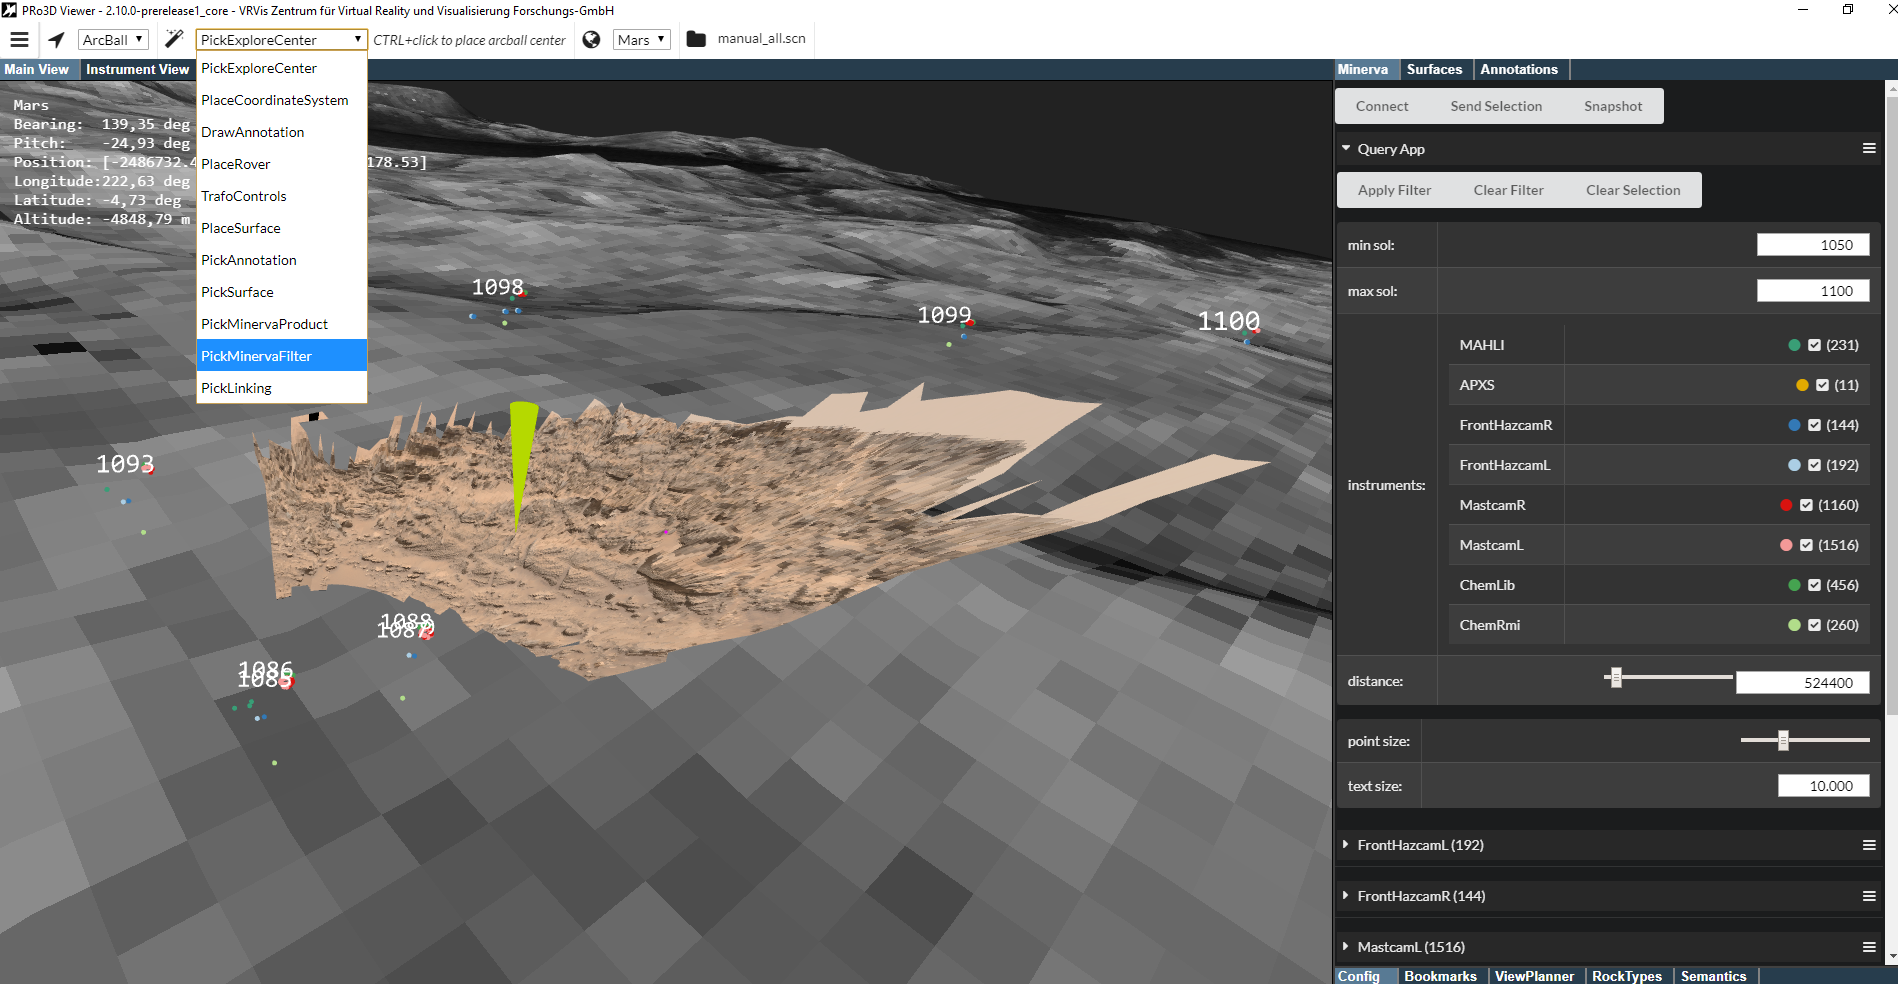
\includegraphics[width=1\textwidth]{pics/PickMinervaFilter.png}
				\caption[Pick Minerva Filter]{PickMinervaFilter}
				\label{fig:PickMinervaFilter}
		 \end{figure}
		
\begin{figure}[h]
				\centering
					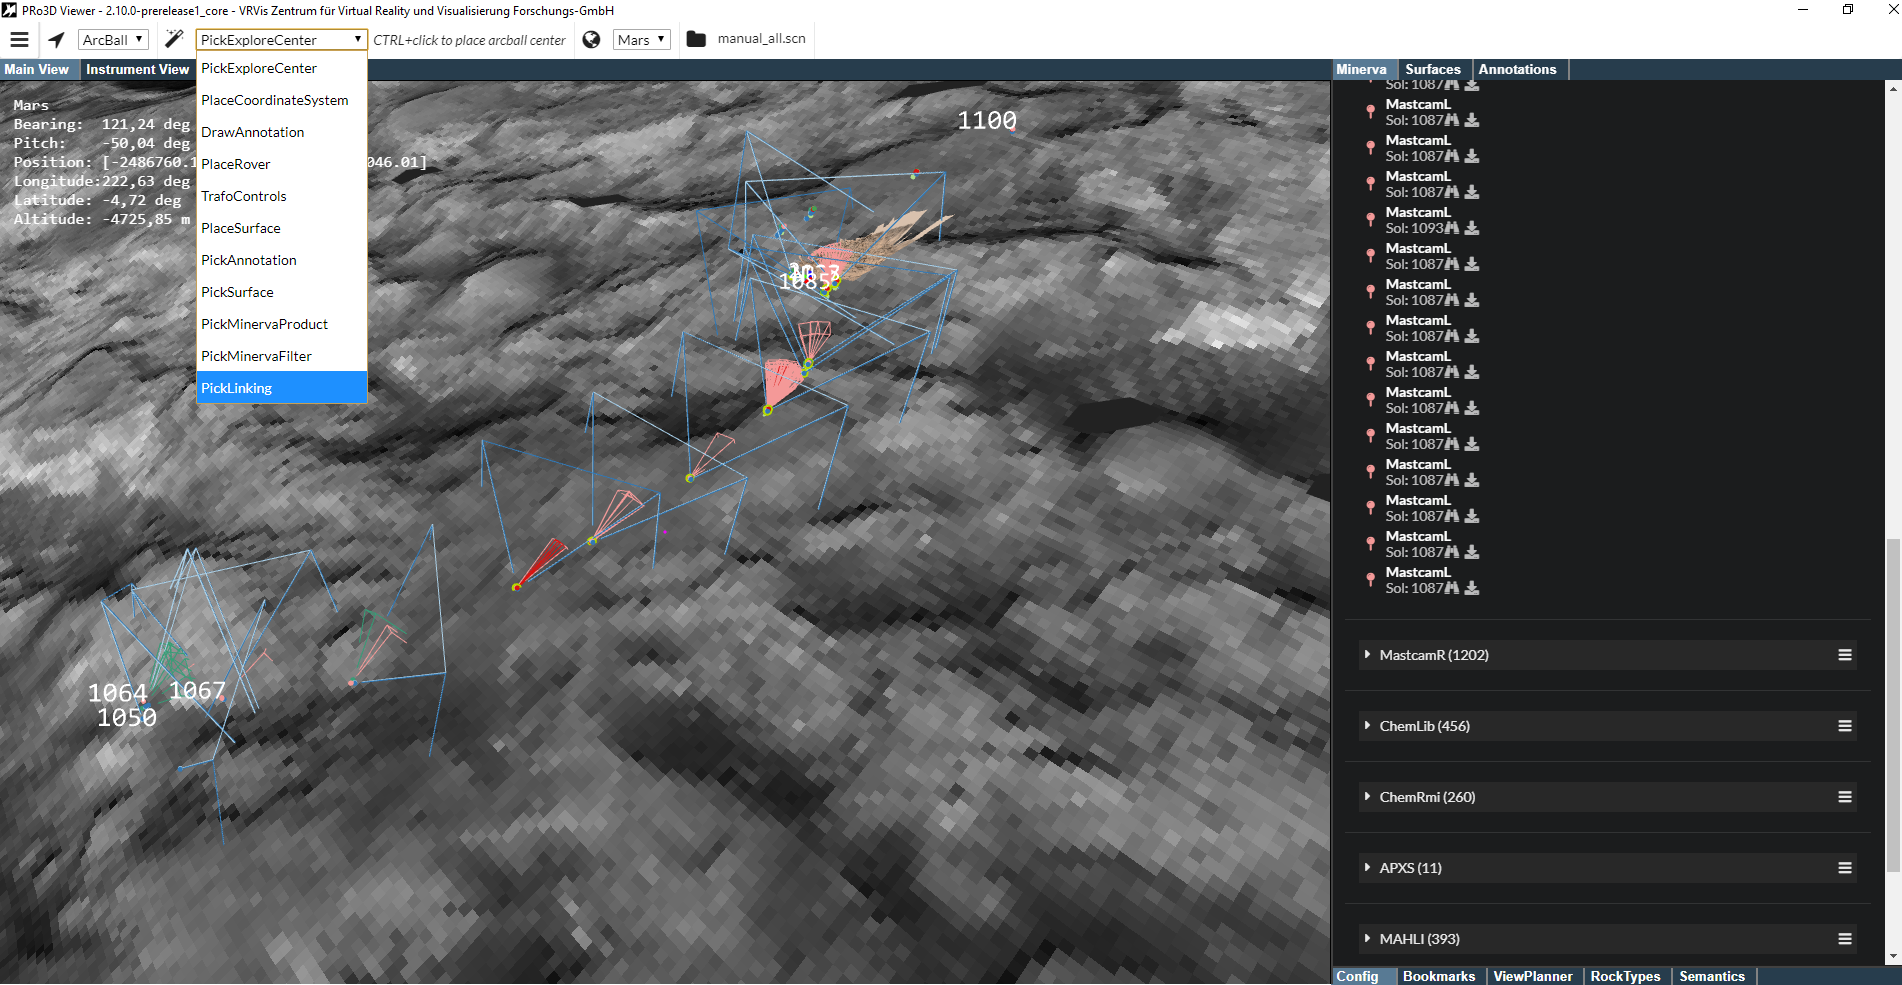
\includegraphics[width=1\textwidth]{pics/PickLinking1.png}
				\caption[Pick Linking]{PickLinking}
				\label{fig:PickLinking}
		 \end{figure}
		

There are three minerva picking actions in the picking actions drop down menu shown in Figure~\ref{fig:PickLinking}.
\\
\begin{itemize}
  \item \textbf{PickMinervaProduct}: You can set ``PickMinervaProduct'' in the actions menu to select a product in the Main View as described in Section~\ref{sec:selection}.
	\item \textbf{PickMinervaFilter}: Select ``PickMinervaFilter'' in the actions menu and press CTRL+LMB to pick a point on the surface. Then set a distance value with the distance slider in the Query App and click the ``ApplyFilter'' button. The products where the distance to the selected point is smaller than the selected distance in the Query App are shown (Figure~\ref{fig:PickMinervaFilter}).
	\item \textbf{PickLinking}: Select ``PickLinking'' in the actions menu and press CTRL+LMB to pick a point on the surface. All camera frustums of the products that captures the selected point are shown (Figure~\ref{fig:PickLinking}).
\end{itemize}

